% -*- mode: latex; coding: utf-8 -*-
\newcommand{\drawblock}[5]{% PARAMETERS: COLOR, CORNERCOORDS, SIZE
% TOP SIDE
\color{#1!55}
\pgfmoveto{\pgfrelative{\pgfxyz(#2,#3,#4)}{\pgfxyz(0,#5,0)}}
\pgflineto{\pgfrelative{\pgfxyz(#2,#3,#4)}{\pgfxyz(#5,#5,0)}}
\pgflineto{\pgfrelative{\pgfxyz(#2,#3,#4)}{\pgfxyz(#5,#5,#5)}}
\pgflineto{\pgfrelative{\pgfxyz(#2,#3,#4)}{\pgfxyz(0,#5,#5)}}
\pgflineto{\pgfrelative{\pgfxyz(#2,#3,#4)}{\pgfxyz(0,#5,0)}}
\pgffill
\color{black}
\pgfmoveto{\pgfrelative{\pgfxyz(#2,#3,#4)}{\pgfxyz(0,#5,0)}}
\pgflineto{\pgfrelative{\pgfxyz(#2,#3,#4)}{\pgfxyz(#5,#5,0)}}
\pgflineto{\pgfrelative{\pgfxyz(#2,#3,#4)}{\pgfxyz(#5,#5,#5)}}
\pgflineto{\pgfrelative{\pgfxyz(#2,#3,#4)}{\pgfxyz(0,#5,#5)}}
\pgflineto{\pgfrelative{\pgfxyz(#2,#3,#4)}{\pgfxyz(0,#5,0)}}
\pgfstroke
% RIGHT SIDE
\color{#1!65}
\pgfmoveto{\pgfrelative{\pgfxyz(#2,#3,#4)}{\pgfxyz(#5,0,0)}}
\pgflineto{\pgfrelative{\pgfxyz(#2,#3,#4)}{\pgfxyz(#5,#5,0)}}
\pgflineto{\pgfrelative{\pgfxyz(#2,#3,#4)}{\pgfxyz(#5,#5,#5)}}
\pgflineto{\pgfrelative{\pgfxyz(#2,#3,#4)}{\pgfxyz(#5,0,#5)}}
\pgflineto{\pgfrelative{\pgfxyz(#2,#3,#4)}{\pgfxyz(#5,0,0)}}
\pgffill
\color{black}
\pgfmoveto{\pgfrelative{\pgfxyz(#2,#3,#4)}{\pgfxyz(#5,0,0)}}
\pgflineto{\pgfrelative{\pgfxyz(#2,#3,#4)}{\pgfxyz(#5,#5,0)}}
\pgflineto{\pgfrelative{\pgfxyz(#2,#3,#4)}{\pgfxyz(#5,#5,#5)}}
\pgflineto{\pgfrelative{\pgfxyz(#2,#3,#4)}{\pgfxyz(#5,0,#5)}}
\pgflineto{\pgfrelative{\pgfxyz(#2,#3,#4)}{\pgfxyz(#5,0,0)}}
\pgfstroke
%FRONT
\color{#1!99}
\pgfmoveto{\pgfxyz(#2,#3,#4)}
\pgflineto{\pgfrelative{\pgfxyz(#2,#3,#4)}{\pgfxyz(#5,0,0)}}
\pgflineto{\pgfrelative{\pgfxyz(#2,#3,#4)}{\pgfxyz(#5,#5,0)}}
\pgflineto{\pgfrelative{\pgfxyz(#2,#3,#4)}{\pgfxyz(0,#5,0)}}
\pgflineto{\pgfxyz(#2,#3,#4)}
\pgffill
\color{black}
\pgfmoveto{\pgfxyz(#2,#3,#4)}
\pgflineto{\pgfrelative{\pgfxyz(#2,#3,#4)}{\pgfxyz(#5,0,0)}}
\pgflineto{\pgfrelative{\pgfxyz(#2,#3,#4)}{\pgfxyz(#5,#5,0)}}
\pgflineto{\pgfrelative{\pgfxyz(#2,#3,#4)}{\pgfxyz(0,#5,0)}}
\pgflineto{\pgfxyz(#2,#3,#4)}
\pgfstroke
}

\newcommand{\RsGsB}{\begin{pgfpicture}{0.5mm}{0.5mm}{12mm}{5mm}
\pgfsetxvec{\pgfpoint{0.4cm}{0cm}}
\pgfsetyvec{\pgfpoint{0cm}{0.4cm}}
\pgfsetzvec{\pgfpoint{0.15cm}{0.15cm}}
\drawblock{red}{0}{0}{0}{1}
\drawblock{green}{1}{0}{0}{1}
\drawblock{blue}{2}{0}{0}{1}
\end{pgfpicture}
}

\newcommand{\twostacksA}[3]{\begin{pgfpicture}{0.5mm}{0.5mm}{0.8cm}{0.9cm}
\pgfsetxvec{\pgfpoint{0.4cm}{0cm}}
\pgfsetyvec{\pgfpoint{0cm}{0.4cm}}
\pgfsetzvec{\pgfpoint{0.15cm}{0.15cm}}
\drawblock{#2}{0}{0}{0}{1}
\drawblock{#1}{0}{1}{0}{1}
\drawblock{#3}{1}{0}{0}{1}
\end{pgfpicture}
}

\newcommand{\twostacksB}[3]{\begin{pgfpicture}{0.5mm}{0.5mm}{0.8cm}{0.9cm}
\pgfsetxvec{\pgfpoint{0.4cm}{0cm}}
\pgfsetyvec{\pgfpoint{0cm}{0.4cm}}
\pgfsetzvec{\pgfpoint{0.15cm}{0.15cm}}
\drawblock{#1}{0}{0}{0}{1}
\drawblock{#3}{1}{0}{0}{1}
\drawblock{#2}{1}{1}{0}{1}
\end{pgfpicture}
}

\newcommand{\onestack}[3]{\begin{pgfpicture}{0.5mm}{0.5mm}{4mm}{13mm}
\pgfsetxvec{\pgfpoint{0.4cm}{0cm}}
\pgfsetyvec{\pgfpoint{0cm}{0.4cm}}
\pgfsetzvec{\pgfpoint{0.15cm}{0.15cm}}
\drawblock{#3}{0}{0}{0}{1}
\drawblock{#2}{0}{1}{0}{1}
\drawblock{#1}{0}{2}{0}{1}
\end{pgfpicture}
}

\newcommand{\RGsB}{\twostacksA{red}{green}{blue}}

\newcommand{\RBsG}{\twostacksB{green}{red}{blue}}
\newcommand{\RBsGr}{\twostacksA{red}{blue}{green}}

\newcommand{\BRsG}{\twostacksA{blue}{red}{green}}
\newcommand{\BRsGr}{\twostacksB{green}{blue}{red}}

\newcommand{\RsBG}{\twostacksB{red}{blue}{green}}

\newcommand{\GRsB}{\twostacksA{green}{red}{blue}}
\newcommand{\RsGB}{\twostacksB{red}{green}{blue}}

\newcommand{\RGB}{\onestack{red}{green}{blue}}
\newcommand{\RBG}{\onestack{red}{blue}{green}}
\newcommand{\GRB}{\onestack{green}{red}{blue}}
\newcommand{\GBR}{\onestack{green}{blue}{red}}
\newcommand{\BRG}{\onestack{blue}{red}{green}}
\newcommand{\BGR}{\onestack{blue}{green}{red}}

%\documentclass{gkibeamer}
\documentclass{beamer}

\usepackage{tikz}
\usepackage{ifthen}
\usepackage{stmaryrd}
\usepackage[T1]{fontenc}
\usepackage[brazil]{babel}
\usepackage[utf8]{inputenc}
%\usetheme{Inf}
%\usetheme{}
\usecolortheme{rose}

%\setbeamertemplate{footline}[frame number]
\setbeamertemplate{footline}{%
  \begin{beamercolorbox}[wd=\paperwidth,ht=2.25ex,dp=2ex]{author in head/foot}%
    \usebeamerfont{author in head/foot}%
    \hfill 
    \hspace*{1em} \insertframenumber\hspace*{1em} % Only display current page number
  \end{beamercolorbox}%
}

\setbeamertemplate{navigation symbols}{}

\title[Discovering and Learning Preferred Operators]{Discovering and Learning Preferred Operators for Classical Planning with Neural Networks}
\author{Pedro Probst Minini}

%\institute{Federal University of Rio Grande do Sul\\Institute of Informatics\\Department of Theoretical Informatics}
%\subject{AI}

\newcommand{\bs}{\texttt{\char`\\}} %% backslash in tt font
\newcommand{\us}{\texttt{\char`_}} %% underscore in tt font

%% Indentation and other things for algorithms
\newcommand{\comment}[1]{\hspace*{\fill}\hilite{[#1]}}
%% for pseudo-code comments
\newcommand{\keyword}[1]{\ensuremath{\textup{\textbf{#1}}}}
\newcommand{\func}[1]{\ensuremath{\textup{#1}}}
%% for pseudo-code
\newcommand{\var}[1]{\ensuremath{\textit{#1}}}
%% for pseudo-code and math variables
\newcommand{\val}[1]{\ensuremath{\textup{#1}}}
%% for values in a finite-domain variable's domain
\newcommand{\op}[1]{\ensuremath{\textit{#1}}}
%% for actions in action sequences in plans etc. (note that \action is
%% already used by LaTeX or some package)

\newcommand{\ind}{{}\qquad}
\newcommand{\indtwo}{\ind\qquad}
\newcommand{\indthree}{\indtwo\qquad}
\newcommand{\indfour}{\indthree\qquad}
\newcommand{\indfive}{\indfour\qquad}

%% Space-saving version of center environment.
\newenvironment{tightcenter}{\centering}{}

%% Math environments
\newenvironment{tightalign}[1][c]{\par\(\begin{array}[#1]{@{}r@{}l}}
               {\end{array}\)\par}
\newenvironment{tightalignnopar}[1][c]{\(\begin{array}[#1]{@{}r@{}l}}
               {\end{array}\)}
\newenvironment{wrappedmath}[1][t]{\begin{array}[#1]{@{}l}}{\end{array}}

%% Don't use proof environment for start of proof since that
%% automatically adds a qed symbol at the end.
\newenvironment{proofstart}{\begin{block}{Proof.}}{\hspace*{\fill}\dots\end{block}}
\newenvironment{proofmiddle}{\begin{block}{Proof (continued).}}{\hspace*{\fill}\dots\end{block}}
\newenvironment{proofend}{\begin{proof}[Proof (continued).]}{\end{proof}}
\newenvironment{proofsketch}{\begin{block}{Proof Sketch.}}{\end{block}}
\newenvironment{proofsketchstart}{\begin{block}{Proof Sketch.}}{\hspace*{\fill}\dots\end{block}}
\newenvironment{proofsketchmiddle}{\begin{block}{Proof Sketch (continued).}}{\hspace*{\fill}\dots\end{block}}
\newenvironment{proofsketchend}{\begin{proof}[Proof Sketch (continued).]}{\end{proof}}
\newcommand{\tbc}{\hspace*{\fill}\dots}

\newtheorem{proposition}{Proposition}

%% Basic text stuff

\newcommand{\hilite}[1]{\textcolor{structure.fg}{#1}}

\newcommand{\ie}{i.e.}
\newcommand{\eg}{e.g.}

\newcommand{\grey}[1]{\textcolor{lightgray}{#1}}
\newcommand{\textred}[1]{{\color{red} #1}}
\newcommand{\orange}[1]{{\color{orange} #1}}
\newcommand{\textblue}[1]{{\color{blue} #1}}
\definecolor{green}{HTML}{28cd4c}
\newcommand{\textgreen}[1]{{\color{green} #1}}
\newcommand{\textorange}[1]{{\color{orange} #1}}

%% Algorithms, mathematical notation etc.

\newcommand{\hstar}{\ensuremath{h^*}}
\newcommand{\rstar}{\ensuremath{r^*}}
\newcommand{\astar}{\ensuremath{\textup{A}^*}}
\newcommand{\idastar}{\ensuremath{\textup{IDA}^*}}
\newcommand{\dom}{\textup{dom}}
\newcommand{\sasplus}{\ensuremath{\textup{SAS}^+}}

\newcommand{\true}{\ensuremath{\mathbf{T}}}
\newcommand{\false}{\ensuremath{\mathbf{F}}}

%\newcommand{\pre}{\ensuremath{\textit{pre}}}
%\newcommand{\eff}{\ensuremath{\textit{eff}}}
\newcommand{\cost}{\ensuremath{\textit{cost}}}
%\newcommand{\add}{\ensuremath{\textit{add}}}
%\newcommand{\del}{\ensuremath{\textit{del}}}
%\newcommand{\precond}{\ensuremath{\textit{prec}}}

\newcommand{\applyop}[2]{#2\llbracket#1\rrbracket}
\newcommand{\applyplan}[2]{#2\llbracket#1\rrbracket}
%% These macros should no longer be used.
%% TODO: Remove them entirely rather than commenting them out once
%% we're happy with our revisions of the parts that used to use them.
%% \newcommand{\changes}[2]{\lbrack #1\rbrack_{#2}}
%% \newcommand{\addchanges}[2]{\lbrack #1\rbrack^+_{#2}}
%% \newcommand{\delchanges}[2]{\lbrack #1\rbrack^-_{#2}}
\newcommand{\condeff}{\vartriangleright}

\newcommand{\addset}{\ensuremath{\textit{addset}}}
\newcommand{\delset}{\ensuremath{\textit{delset}}}

\newcommand{\effcond}{\ensuremath{\textit{effcond}}}
\newcommand{\consist}{\ensuremath{\textit{consist}}}

\newcommand{\vars}{\ensuremath{\textit{vars}}}

\newcommand{\regr}{\ensuremath{\textit{regr}}}
\newcommand{\regrstrips}{\ensuremath{\textit{sregr}}}
\newcommand{\eprecon}[2]{\textit{EPC}_{#1}(#2)}
\newcommand{\sregrpairs}[2]{R(#2, #1)}
\newcommand{\varset}[1]{\ensuremath{\textit{vars}(#1)}}
\newcommand{\conj}[1]{\ensuremath{\textit{conj}(#1)}}

%% Blocks world examples
\newcommand{\AONB}{\var{A-on-B}}
\newcommand{\AONC}{\var{A-on-C}}
\newcommand{\AOND}{\var{A-on-D}}
\newcommand{\BONA}{\var{B-on-A}}
\newcommand{\BONC}{\var{B-on-C}}
\newcommand{\BOND}{\var{B-on-D}}
\newcommand{\CONA}{\var{C-on-A}}
\newcommand{\CONB}{\var{C-on-B}}
\newcommand{\COND}{\var{C-on-D}}
\newcommand{\DONA}{\var{D-on-A}}
\newcommand{\DONB}{\var{D-on-B}}
\newcommand{\DONC}{\var{D-on-C}}
\newcommand{\AONTABLE}{\var{A-on-table}}
\newcommand{\BONTABLE}{\var{B-on-table}}
\newcommand{\CONTABLE}{\var{C-on-table}}
\newcommand{\CLEARA}{\var{A-clear}}
\newcommand{\CLEARB}{\var{B-clear}}
\newcommand{\CLEARC}{\var{C-clear}}

%% Macros to align the width of things.
\newlength{\mywidth}
\newcommand{\setmywidth}[1]{\settowidth{\mywidth}{#1}}
\newcommand{\usemywidth}[1]{\makebox[\mywidth][l]{#1}}
\newcommand{\usemywidthmath}[1]{\usemywidth{\ensuremath{#1}}}

\newcounter{mysaveenumi}
\newcommand{\enumtbc}{\setcounter{mysaveenumi}{\theenumi}}
\newcommand{\continueenum}{\setcounter{enumi}{\themysaveenumi}}

%% Complexity classes.
\newcommand{\decisionclass}[1]{\ensuremath{\textsf{\textup{#1}}}}
\newcommand{\dtime}{\decisionclass{DTIME}}
\newcommand{\ntime}{\decisionclass{NTIME}}
\newcommand{\dspace}{\decisionclass{DSPACE}}
\newcommand{\nspace}{\decisionclass{NSPACE}}
\newcommand{\ptime}{\decisionclass{P}}
\newcommand{\np}{\decisionclass{NP}}
\newcommand{\pspace}{\decisionclass{PSPACE}}
\newcommand{\npspace}{\decisionclass{NPSPACE}}
\newcommand{\exptime}{\decisionclass{EXP}}
\newcommand{\expspace}{\decisionclass{EXPSPACE}}
\newcommand{\dblexptime}{\decisionclass{2-EXP}}
\newcommand{\dblexpspace}{\decisionclass{2-EXPSPACE}}

%% Turing machine stuff.
\newcommand{\accept}{{\textsf{Y}}}

%% Decision problems and related things.
\newcommand{\planex}{\textsc{PlanEx}}
\newcommand{\bcplanex}{\textsc{BCPlanEx}}
\newcommand{\easier}{\ensuremath{\le_{\text{p}}}}

%% Various stuff.
\newcommand{\relaxation}[1]{#1^+}
\newcommand{\onset}[1]{\textit{on}(#1)}

%% Heuristics.
\newcommand{\hplus}{\ensuremath{h^+}}
\newcommand{\hmax}{\ensuremath{h^{\text{max}}}}
\newcommand{\hadd}{\ensuremath{h^{\text{add}}}}
\newcommand{\hlmcut}{\ensuremath{h^{\text{LM-cut}}}}
\newcommand{\hff}{\ensuremath{h^{\text{FF}}}}
\newcommand{\hcs}{\ensuremath{h^{\text{cs}}}}
\newcommand{\hsa}{\ensuremath{h^{\text{sa}}}}
\newcommand{\hlst}{\ensuremath{h^{\text{lst}}}}
\newcommand{\hm}{\ensuremath{h^m}}
\newcommand{\hmhs}{\ensuremath{h^\text{MHS}}}
\newcommand{\hucp}{\ensuremath{h^\text{UCP}}}
\newcommand{\hlmcount}{\ensuremath{h^\text{LM-count}}}
\newcommand{\hflow}{\ensuremath{h^\text{flow}}}
\newcommand{\hposthoc}[1][]{\ensuremath{h_{#1}^{\textup{PhO}}}}
\newcommand{\hcanon}{\ensuremath{h^{\mathcal{C}}}}
\newcommand{\hocp}{\ensuremath{h^\textup{OCP}}}

%% Used for AND/OR graphs.
%% Note that \succ is already used by LaTeX.
\newcommand{\suc}{\ensuremath{\textit{succ}}}

%% Used for abstraction chapters.
\newcommand{\graphequiv}{\stackrel{\textup{G}}{\sim}}
\newcommand{\cg}{\ensuremath{\textit{CG}}}
\newcommand{\hhhh}{\ensuremath{h_{\text{HHH}}}}

\newcommand{\cliques}{\ensuremath{\textit{cliques}}}

% AND/OR landmarks
\newcommand{\andorarc}[2]{\ensuremath{\langle #1,#2\rangle}}
\newcommand{\landmark}{\textit{LM}}

% Landmark orderings
\newcommand{\naturalord}[2]{\ensuremath{#1\rightarrow #2}}
\newcommand{\necessaryord}[2]{\ensuremath{#1\rightarrow_{\textup{n}} #2}}
\newcommand{\greedynecessaryord}[2]{\ensuremath{#1\rightarrow_{\textup{gn}} #2}}
\newcommand{\arbitraryord}[2]{\ensuremath{#1\rightarrow_{\textup{x}} #2}}


\newcommand{\lpvar}[1]{\ensuremath{\hilite{#1}}}
\newcommand{\ocvar}[1]{\lpvar{\textup{Count}_{#1}}}

\providecommand{\floor}[1]{\ensuremath{\left\lfloor #1\right\rfloor}}
\providecommand{\ceil}[1]{\ensuremath{\left\lceil #1\right\rceil}}


\providecommand{\multiset}[1]{\ensuremath{\{\!\!\{#1\}\!\!\}}}
\providecommand{\sas}{\ensuremath{\text{SAS}^{+}}\xspace}
\providecommand{\strips}{STRIPS\xspace}
\providecommand{\astar}{\ensuremath{\text{A}^{*}}\xspace}
\providecommand{\gbfs}{\ensuremath{\text{GBFS}}\xspace}
\providecommand{\wida}{\ensuremath{\text{W-IDA}^{*}}\xspace}
\providecommand{\ida}{\ensuremath{\text{IDA}^{*}}\xspace}
\providecommand{\hvalue}[1]{\ensuremath{h^{#1}}\xspace}
\providecommand{\hstarp}[1]{\ensuremath{h^*({#1})}\xspace}
\providecommand{\hff}{\hvalue{\text{FF}}}
\providecommand{\hgc}{\hvalue{\text{GC}}}
\providecommand{\hstar}{\hvalue{*}}
\providecommand{\hlmc}{\hvalue{\text{lm-c}}}
\providecommand{\hmax}{\hvalue{\text{max}}}
\providecommand{\hadd}{\hvalue{\text{add}}}
\providecommand{\hblind}{\hvalue{\text{blind}}}
\providecommand{\h}{$h$\xspace}
\providecommand{\hnn}{$\hat h$\xspace}
\providecommand{\hnrsl}{$\hat h^{\text{N-RSL}}$\xspace}
\providecommand{\hboot}{$\hat h^{\text{Boot}}$\xspace}
\providecommand{\hgc}{\hvalue{\text{gc}}}
\providecommand{\hhgn}{\hvalue{\text{HGN}}}
\providecommand{\unit}{/1\xspace}
\providecommand{\sui}{\text{SUI}\xspace}
\providecommand{\sai}{\text{SAI}\xspace}
\providecommand{\rw}{{RW}\xspace}
\providecommand{\bfs}{{BFS}\xspace}
\providecommand{\dfs}{{DFS}\xspace}
\providecommand{\bfsrw}{\text{FSM}\xspace}
\providecommand{\bfsrs}{\text{XRS}\xspace}
\providecommand{\nn}{{NN}\xspace}
\providecommand{\spp}{{\text{SP}}\xspace}
\providecommand{\fsp}{{\text{FSP}}\xspace}
\providecommand{\bsp}{{\text{BSP}}\xspace}
\providecommand{\hnnrs}{$\hat h{^{20\%}_\text{\meanfx}}$\xspace}
\providecommand{\hnnrsfifty}{$\hat h{^{50\%}_\text{\meanfx}}$\xspace}
\providecommand{\hffexp}{$h^{FF}_{exp}$}
\providecommand{\hgcexp}{$h^{GC}_{exp}$}
\providecommand{\hnnbase}{$\hat h_{0}$\xspace}
\providecommand{\hnnbfs}{$\hat h_{\text{bfs}}$\xspace}
\providecommand{\hnndfs}{$\hat h_{\text{dfs}}$\xspace}
\providecommand{\hnnrw}{$\hat h_{\text{rw}}$\xspace}
\providecommand{\hnnbfsrw}{$\hat h_\text{fsm}$\xspace}
\providecommand{\hnnbfsrwl}[1]{\ensuremath{\hat h_{#1}}\xspace}
\providecommand{\hnnnomutex}{\ensuremath{\hat h^{'}}\xspace}
\providecommand{\hnnnomutexl}[1]{\ensuremath{\hat h^{'}_{#1}}\xspace}
\providecommand{\hnnrsp}[1]{\ensuremath{\hat h_\text{fsm}/^{#1\%}_{\text{RS}}}\xspace}
\providecommand{\hnnrslp}[2]{\ensuremath{\hat h_\text{fsm}^{#1}/^{#2\%}_{\text{RS}}}\xspace}
\providecommand{\define}[1]{#1}
\providecommand{\facts}{\ensuremath{L_F}\xspace}
\providecommand{\meanfx}{\ensuremath{L_{\overline{F}}}\xspace}
\providecommand{\default}{\ensuremath{L_{200}}\xspace}
\providecommand{\distfarthest}{\ensuremath{d^*}\xspace}
\providecommand{\po}[1]{\ensuremath{\hat po^{#1}}\xspace}
\providecommand{\pot}[1]{\ensuremath{po^{#1}}\xspace}
\providecommand{\pog}{\po{\text{G}}}
\providecommand{\pofsm}{\po{\text{FSM}}}
\providecommand{\pogthresh}{\po{\text{G-thresh}}}
\providecommand{\pogmax}{\po{\text{G-max}}}
\providecommand{\popfa}{\po{\text{PFA}}}
\providecommand{\popfo}{\po{\text{PFO}}}
\providecommand{\postar}{\po{*}}
\providecommand{\postartable}{\pot{*}}
\providecommand{\pogstar}{\po{\text{G}^*}}
\providecommand{\pogstarthresh}{\po{\text{OPT-thresh}}}
\providecommand{\pogstarmax}{\po{\text{OPT-max}}}
\providecommand{\popf}{\po{\text{PF}}}
\providecommand{\poff}{\pot{\text{FF}}}
\providecommand{\pogc}{\po{\text{GC}}}

%% mathematical definitions
\ifcsname dom\endcsname\else\DeclareMathOperator{\dom}{dom}\fi
\DeclareMathOperator{\pre}{pre}
\DeclareMathOperator{\eff}{eff}
\DeclareMathOperator{\sucs}{succ}
\DeclareMathOperator{\pred}{pred}
\DeclareMathOperator{\functioninitial}{initial\_state}
\DeclareMathOperator{\functiongoal}{goal\_condition}
\DeclareMathOperator{\mutex}{mutex}
\DeclareMathOperator{\del}{del}
\DeclareMathOperator{\add}{add}
\ifcsname R\endcsname\else\newcommand{\R}{\ensuremath{\mathbb{R}}}\fi


% #############################################################################################################
%
%% Needed for "Content of this Course" slide in most chapters:
\usetikzlibrary{positioning, calc, decorations.pathreplacing, arrows, arrows.meta, patterns, automata}
\usepackage[outline]{contour} % glow around text
\contourlength{1.4pt}
\tikzset{>=latex} % for LaTeX arrow head
\colorlet{myred}{red!80!black}
\colorlet{myblue}{blue!80!black}
\colorlet{mygreen}{green!60!black}
\colorlet{myorange}{orange!70!red!60!black}
\colorlet{mydarkred}{red!30!black}
\colorlet{mydarkblue}{blue!40!black}
\colorlet{mydarkgreen}{green!30!black}
\tikzset{ % node styles, numbered for easy mapping with \nstyle
  my nodes/.style={circle,inner sep=0,minimum size=8mm},
  input/.style={my nodes,draw=mygreen,fill=mygreen!20,text=green!50!black},
  hidden/.style={my nodes,draw=violet,fill=violet!20,text=violet},
  output/.style={my nodes,draw=myred!60!black,fill=myred!20,text=red!60!black},
  my text/.style={text=#1,text width=1cm,align=center}
}

\usepackage[linesnumbered, ruled, vlined]{algorithm2e}
\usepackage{mathtools}
\usepackage{booktabs}
\usepackage{comment}
\usepackage{multicol}
%\usepackage{natbib}
\usepackage[citestyle=authoryear,maxnames=10,maxcitenames=1,giveninits=true,backend=biber,uniquelist=false]{biblatex}
\usepackage[utf8]{inputenc}
\usepackage[textsize=tiny,colorinlistoftodos,prependcaption]{todonotes}
\addbibresource{biblio.bib}

\newcommand{\pp}[2][noinline]{\todo[color=purple!50,linecolor={purple!100},#1,fancyline,author=Pedro]{#2}}
\newcommand{\ppi}[2][inline]{\todo[color=purple!50,linecolor={purple!100},#1,fancyline,author=Pedro]{#2}}

% #####################
\AtBeginSubsection[]
{
\begin{frame}[noframenumbering]
    %\frametitle{\n}
    \begin{beamercolorbox}[sep=8pt,center,shadow=true,rounded=true]{title}
      \usebeamerfont{title}\insertsectionhead\par%
    \end{beamercolorbox}
    \tableofcontents[currentsection,currentsubsection]
\end{frame}
}

\AtBeginSection[]{
  \begin{frame}
    \setbeamercolor{section title}{fg=beamer@blendedblue,bg=structure}
    \usebeamercolor[fg]{section title}
    \centering
    \Huge\insertsectionhead
  \end{frame}
}
% #####################

\addbibresource{biblio.bib}

% #############################################################################################################

%\subtitle{Some title}
%\date{}
%\begin{document}

%\begin{frame}{Outline}
%\tableofcontents
%\end{frame}

% Define the title with \title[short title]{long title}
% Short title is optional
\title[Discovering and Learning Preferred Operators]
      {Discovering and Learning Preferred Operators for Classical Planning with Neural Networks}

% Optional subtitle
%\subtitle{Defesa de Mestrado}

\date{Julho de 2023}

% Author information
\author{Pedro Probst Minini}
\institute{Instituto de Informática --- UFRGS}

\begin{document}

% Command to create title page (INF)
%\InfTitlePage

\begin{frame}[plain]
  \titlepage
\end{frame}

\begin{frame}{Outline}
  \frametitle{Agenda}
  \tableofcontents
\end{frame}

\section{Problema}
\begin{frame}{O Que Queremos Fazer?}
Planejadores que usam operadores preferidos para \alert{priorizar a expansão de estados mais promissores} foram os vencedores da trilha \emph{satisficing} da \emph{International Planning Competition} (IPC) em \alert{2004}~(\cite{Helmert/2006}), \alert{2008}~(\cite{Richter.lama.etal/2010}), \alert{2011}~(\cite{Richter.lama.etal/2011}), and \alert{2018}~(\cite{Seipp-fast.etal/2018}).

\pause
\begin{itemize}
  \item Abordagens existentes para a derivação de operadores preferidos são baseadas em lógica (e.g. operadores preferidos do FF).
  \pause
  \item Há vários métodos para o aprendizado de funções heurísticas usando redes neurais.
  \begin{itemize}
    \item Mas nada sobre aprender operadores preferidos.
  \end{itemize}
\end{itemize}
\end{frame}

\begin{frame}{O Que Queremos Fazer?}
\begin{itemize}
  \item Propomos um método para gerar amostras de estados, onde \alert{cada estado tem um conjunto de operadores preferidos}.
  \pause
  \item Usamos esses conjuntos de amostras gerados para \alert{treinar redes neurais} que, durante a resolução de um problema de planejamento, escolhem operadores preferidos para o estado atual.
\end{itemize}
\pause
\begin{align*}
\centering
&(\text{valor-}h;\text{estado};POs) \\
&16;00000001011110110\ldots0000000100000001;71 \\
&17;00000001010110100\ldots0000000100000001;8,20 \\
&\ldots \\
&13;00000001000101101\ldots0000010000100000;7 \\
&14;00000001010100110\ldots0000010000100000;93,60 \\
&13;00000001011100000\ldots0000010010000000;13 \\
&\ldots
\end{align*}
\end{frame}


\section{Introdução}

\subsection{Planejamento}
\begin{frame}{Planejamento Clássico}
\emph{Planejamento} tem o objetivo de encontrar uma \alert{sequência de ações} a partir de um \alert{estado inicial} que satisfaça as \alert{condições objetivo}.
    \begin{exampleblock}{\strut Exemplo: Planejamento Clássico}
      \hilite{ambiente}
      \begin{itemize}
      \item \alert{estático} vs.\ \grey{dinâmico}
        \pause
      \item \alert{determinístico} vs.\ \grey{não determinístico}
        vs.\ \grey{estocástico}
        \pause
      \item \alert{observável}
        vs.\ \grey{parcialmente observável}
        vs.\ \grey{não observável}
        \pause
      \item \alert{discreto} vs.\ \grey{contínuo}
        \pause
      \item \alert{agente único} vs.\ \grey{agentes multiplos}
      \end{itemize}

      \pause
      \hilite{método de resolução}
      \begin{itemize}
      \item \grey{específico por problema} vs.\ \alert{geral} vs.\ \orange{aprendizado}
      \end{itemize}
    \end{exampleblock}
% ppi{Then briefly talk about non-deterministic planning.}
% Classical Planning is an example of a "model".
\end{frame}

\begin{frame}{STRIPS}
  \begin{definition}[Um problema de planejamento em STRIPS]
    $\Pi = \langle F, O, s_{0}, s^{*}\rangle$ onde
    \begin{itemize}
        \item $F$ é um conjunto de variáveis booleanas (\alert{fatos} ou \alert{proposições}),
        \item $O$ é um conjunto de \alert{operadores} ou ações sobre $F$, onde $\langle pre(o), add(o), del(o) \rangle \subseteq F$,
        \item $s_{0} \subseteq F$ é o conjunto de fatos que representa o \alert{estado inicial}, e
        \item $s^{*} \subseteq F$ é o conjunto de fatos que devem ser satisfeitos (``\alert{gol}'').
    \end{itemize}
   \pause
    As ações $A(s)$ são \alert{aplicáveis} em $s$ se elas satisfizerem $pre(o)$.

    Avançamos de um estado $s$ com o operador $o$ definindo as proposições em $add(o)$ como \alert{verdadeiras} e em $del(o)$ como \alert{falsas}.
    %\pause
    %Por fim, $\pi = o_{1}, o_{2},\ldots, o_{n}$ é chamado de \alert{plano} para $\Pi$, em que $o_{i}$ é um operador aplicável.
\end{definition}
%Planning tasks are usually formally described in PDDL files, following a Lisp-like structure.
\end{frame}

\begin{frame}{Example: Blocksworld} 
\begin{figure}
    \centering
    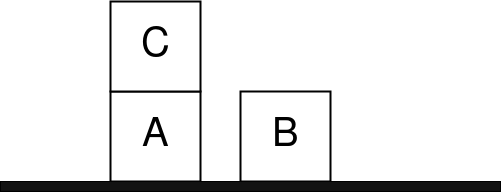
\includegraphics[width=7cm]{img/blocksworld1.png}
    \caption{Uma tarefa de planejamento do domínio Blocks World.}
\end{figure}
\end{frame}

\begin{frame}{Exemplo: Blocksworld}
% This is from Malte Helmert's slides, slightly modified.
    \begin{exampleblock}{\strut Exemplo: Blocks World}
      \hilite{$\Pi = \langle F, O, s_{0}, s^{*}\rangle$}
      \begin{itemize}
      \item $F$ = \{on(a,b), on(a,c), on(b,a), on(b,c), on(c,a), on(c,b), on-table(a), on-table(b), on-table(c), clear(a), clear(b), clear(c)\}

       \item $O$ = \{move(a,b,c), move(a,c,b), move(b,a,c), move(b,c,a), move(c,a,b), move(c,b,a), to-table(a,b), to-table(a,c), to-table(b,a), to-table(b,c), to-table(c,a), to-table(c,b), from-table(a,b), from-table(a,c), from-table(b,a), from-table(b,c), from-table(c,a), from-table(c,b)\}

        \item $s_{0}$ = \{on(c,a), on-table(a), on-table(b), clear(c), clear(b)\}

         \item $s^{*}$ = \{on(a,b), on(b,c)\}
      \end{itemize}
    \end{exampleblock}
\end{frame}

\begin{frame}{Exemplo: Blocks World}
    \begin{exampleblock}{\strut Exemmplo: Blocks World}
      \begin{itemize}
      \item \emph{move}: move a block from one block to another.
      \begin{itemize}
        \item Pre(move(a,b,c)) = \{on(a,b), clear(a), clear(c)\}
        \item Add(move(a,b,c)) = \{on(a,c), clear(b)\}
        \item Del(move(a,b,c)) = \{on(a,b), clear(c)\}
        \item Com base no estado inicial, essa ação é aplicável? % Não, ela não satisfaz as condições prévias.
      \end{itemize}
      \item \emph{to-table}: mover um bloco de um bloco para a mesa.
      \item \emph{from-table}: mover um bloco de um bloco para a mesa.
      \end{itemize}
    \end{exampleblock}
\end{frame}

\begin{frame}{Espaço de Estados do Blocks World com 3 Blocos}
  \begin{center}
    \begin{pgfpicture}{-39mm}{-32.4mm}{39mm}{32.4mm}
      \pgfnodebox{RsGsB}[virtual]{\pgfpolar{0}{0cm}}{\RsGsB}{2pt}{2pt}

      \pgfnodebox{RGsB}[virtual]{\pgfpolar{0}{16mm}}{\RGsB}{2pt}{2pt}
      \pgfnodebox{RBsG}[virtual]{\pgfpolar{60}{16mm}}{\RBsG}{2pt}{2pt}
      \pgfnodebox{BRsG}[virtual]{\pgfpolar{120}{16mm}}{\BRsG}{2pt}{2pt}
      \pgfnodebox{RsBG}[virtual]{\pgfpolar{180}{16mm}}{\RsBG}{2pt}{2pt}
      \pgfnodebox{RsGB}[virtual]{\pgfpolar{240}{16mm}}{\RsGB}{2pt}{2pt}
      \pgfnodebox{GRsB}[virtual]{\pgfpolar{300}{16mm}}{\GRsB}{2pt}{2pt}

      \pgfnodebox{BRG}[virtual]{\pgfpolar{0}{32mm}}{\BRG}{2pt}{2pt}
      \pgfnodebox{GRB}[virtual]{\pgfpolar{50}{32mm}}{\GRB}{2pt}{2pt}
      \pgfnodebox{GBR}[virtual]{\pgfpolar{130}{32mm}}{\GBR}{2pt}{2pt}
      \pgfnodebox{RBG}[virtual]{\pgfpolar{180}{32mm}}{\RBG}{2pt}{2pt}
      \pgfnodebox{RGB}[virtual]{\pgfpolar{230}{32mm}}{\RGB}{2pt}{2pt}
      \pgfnodebox{BGR}[virtual]{\pgfpolar{310}{32mm}}{\BGR}{2pt}{2pt}

      \pgfsetendarrow{\pgfarrowtriangle{5pt}}
      \pgfsetstartarrow{\pgfarrowtriangle{5pt}}

      \pgfnodeconnline{RsGsB}{RGsB}
      \pgfnodeconnline{RsGsB}{RBsG}
      \pgfnodeconnline{RsGsB}{BRsG}
      \pgfnodeconnline{RsGsB}{RsBG}
      \pgfnodeconnline{RsGsB}{RsGB}
      \pgfnodeconnline{RsGsB}{GRsB}

      \pgfnodeconnline{RGsB}{BRG}
      \pgfnodeconnline{RBsG}{GRB}
      \pgfnodeconnline{BRsG}{GBR}
      \pgfnodeconnline{RsBG}{RBG}
      \pgfnodeconnline{RsGB}{RGB}
      \pgfnodeconnline{GRsB}{BGR}

      \pgfnodeconnline{RGsB}{RBsG}
      \pgfnodeconnline{BRsG}{RsBG}
      \pgfnodeconnline{RsGB}{GRsB}
    \end{pgfpicture}
  \end{center}
\end{frame}

\begin{frame}{\sas}
\begin{itemize}
\item \sas é similar a STRIPS, mas variáveis têm domínios finitos, não sendo necessariamente binárias.
  \item O estado inicial $s_{0}$ é tipicamente um \alert{estado completo}, i.e., todas as variáveis estão definidas.
  \item O gol $s^{*}$ é definido \alert{parcialmente}, com certas variáveis indefinidas ($\bot$).
\end{itemize}
\end{frame}

\subsection{Busca Heurística}
\begin{frame}{Busca Heurística}
\begin{itemize}
  \item Planejadores tipicamente buscam satisfazer o gol \alert{priorizando} estados no espaço de estados com \alert{menor função heurística}.
  \pause
  \item Um estado $s$ tem uma função heurística $h(s)$, dado por uma função heurística $h$, que estima o \alert{custo de atingir o gol $s^{*}$} a partir de $s$.
  \pause
  \item Algoritmos ``best-first search'', e.g., greedy best-first serach (GBFS), \astar.
\end{itemize}
\end{frame}

\begin{frame}{Busca Heurística: Exemplo com GBFS}
\only<1> {
\begin{figure}[tb]
\centering
\begin{tikzpicture}
    [
        node distance=21mm and 22mm, on grid, auto, label distance=-0.5mm,
        black_node/.style={circle, draw=black!100, fill=black!0, very thick, minimum height=8mm, minimum width=8mm},
        red_node/.style={circle, draw=red!100, fill=red!0, very thick, minimum height=8mm, minimum width=8mm},
    ]

  \node[black_node,label=above:{\footnotesize$2$}] (A) at (0,0) {\footnotesize$s_0$};
  \node[black_node,label=above:{\footnotesize$3$}] (B) at (-1.7,-1) {\footnotesize$s_{1}$};
  \node[black_node,label=above:{\footnotesize$1$}] (C) at (1.7,-1) {\footnotesize$s_{2}$};
  \node[black_node,label=above:{\footnotesize$4$}] (D) at (-2.7,-2) {\footnotesize$s_{3}$};
  \node[black_node,label=above:{\footnotesize$4$}] (E) at (-0.7,-2) {\footnotesize$s_{4}$};
  \node[black_node,label=above:{\footnotesize$2$}] (F) at (0.7,-2) {\footnotesize$s_{5}$};
  \node[black_node, accepting,label=above:{\footnotesize$0$}] (G) at (2.7,-2) {\footnotesize$s^{*}$};

  \draw (A) -- (B);
  \draw (A) -- (C);
  \draw (B) -- (D);
  \draw (B) -- (E);
  \draw (C) -- (F);
  \draw (C) -- (G);
\end{tikzpicture}
\end{figure}

\begin{table}[b]
\centering
\begin{tabular}{|c|c|}
\hline
\textbf{Iteração} & \textbf{Fila de Prioridades} \\
\hline
0 & ($s_{0}$, 2) \\
\hline
\end{tabular}
\end{table}
}

\only<2> {
\begin{figure}[tb]
\centering
\begin{tikzpicture}
    [
        node distance=21mm and 22mm, on grid, auto, label distance=-0.5mm,
        black_node/.style={circle, draw=black!100, fill=black!0, very thick, minimum height=8mm, minimum width=8mm},
        red_node/.style={circle, draw=red!100, fill=red!0, very thick, minimum height=8mm, minimum width=8mm},
    ]

  \node[red_node,label=above:{\footnotesize$2$}] (A) at (0,0) {\footnotesize$s_0$};
  \node[red_node,label=above:{\footnotesize$3$}] (B) at (-1.7,-1) {\footnotesize$s_{1}$};
  \node[red_node,label=above:{\footnotesize$1$}] (C) at (1.7,-1) {\footnotesize$s_{2}$};
  \node[black_node,label=above:{\footnotesize$4$}] (D) at (-2.7,-2) {\footnotesize$s_{3}$};
  \node[black_node,label=above:{\footnotesize$4$}] (E) at (-0.7,-2) {\footnotesize$s_{4}$};
  \node[black_node,label=above:{\footnotesize$2$}] (F) at (0.7,-2) {\footnotesize$s_{5}$};
  \node[black_node, accepting,label=above:{\footnotesize$0$}] (G) at (2.7,-2) {\footnotesize$s^{*}$};

  \draw[red] (A) -- (B);
  \draw[red] (A) -- (C);
  \draw (B) -- (D);
  \draw (B) -- (E);
  \draw (C) -- (F);
  \draw (C) -- (G);
\end{tikzpicture}
\end{figure}

\begin{table}[b]
\centering
\begin{tabular}{|c|c|}
\hline
\textbf{Iteração} & \textbf{Fila de Prioridades} \\
\hline
0 & ($s_{0}$, 2) \\
\hline
1 & ($s_{2}$, 1) \quad ($s_{1}$, 3) \\
\hline
\end{tabular}
\end{table}
}

\only<3> {
\begin{figure}[b]
\centering
\begin{tikzpicture}
    [
        node distance=21mm and 22mm, on grid, auto, label distance=-0.5mm,
        black_node/.style={circle, draw=black!100, fill=black!0, very thick, minimum height=8mm, minimum width=8mm},
        red_node/.style={circle, draw=red!100, fill=red!0, very thick, minimum height=8mm, minimum width=8mm},
    ]

  \node[black_node,label=above:{\footnotesize$2$}] (A) at (0,0) {\footnotesize$s_0$};
  \node[black_node,label=above:{\footnotesize$3$}] (B) at (-1.7,-1) {\footnotesize$s_{1}$};
  \node[red_node,label=above:{\footnotesize$1$}] (C) at (1.7,-1) {\footnotesize$s_{2}$};
  \node[black_node,label=above:{\footnotesize$4$}] (D) at (-2.7,-2) {\footnotesize$s_{3}$};
  \node[black_node,label=above:{\footnotesize$4$}] (E) at (-0.7,-2) {\footnotesize$s_{4}$};
  \node[red_node,label=above:{\footnotesize$2$}] (F) at (0.7,-2) {\footnotesize$s_{5}$};
  \node[red_node, accepting,label=above:{\footnotesize$0$}] (G) at (2.7,-2) {\footnotesize$s^{*}$};

  \draw[gray] (A) -- (B);
  \draw[gray] (A) -- (C);
  \draw (B) -- (D);
  \draw (B) -- (E);
  \draw[red] (C) -- (F);
  \draw[red] (C) -- (G);
\end{tikzpicture}
\end{figure}

\begin{table}[b]
\centering
\begin{tabular}{|c|c|}
\hline
\textbf{Iteração} & \textbf{Fila de Prioridades} \\
\hline
0 & ($s_{0}$, 2) \\
\hline
1 & ($s_{2}$, 1) \quad ($s_{1}$, 3) \\
\hline
2 & ($s^{*}$, 0) \quad ($s_{5}$, 2) \quad ($s_{1}$, 3) \\
\hline
\end{tabular}
\end{table}
}

\only<4> {
\begin{figure}[b]
\centering
\begin{tikzpicture}
    [
        node distance=21mm and 22mm, on grid, auto, label distance=-0.5mm,
        black_node/.style={circle, draw=black!100, fill=black!0, very thick, minimum height=8mm, minimum width=8mm},
        red_node/.style={circle, draw=red!100, fill=red!0, very thick, minimum height=8mm, minimum width=8mm},
    ]

  \node[black_node,label=above:{\footnotesize$2$}] (A) at (0,0) {\footnotesize$s_0$};
  \node[black_node,label=above:{\footnotesize$3$}] (B) at (-1.7,-1) {\footnotesize$s_{1}$};
  \node[black_node,label=above:{\footnotesize$1$}] (C) at (1.7,-1) {\footnotesize$s_{2}$};
  \node[black_node,label=above:{\footnotesize$4$}] (D) at (-2.7,-2) {\footnotesize$s_{3}$};
  \node[black_node,label=above:{\footnotesize$4$}] (E) at (-0.7,-2) {\footnotesize$s_{4}$};
  \node[black_node,label=above:{\footnotesize$2$}] (F) at (0.7,-2) {\footnotesize$s_{5}$};
  \node[red_node, accepting,label=above:{\footnotesize$0$}] (G) at (2.7,-2) {\footnotesize$s^{*}$};

  \draw[gray] (A) -- (B);
  \draw[red] (A) -- (C);
  \draw (B) -- (D);
  \draw (B) -- (E);
  \draw[gray] (C) -- (F);
  \draw[red] (C) -- (G);
\end{tikzpicture}
\end{figure}

\begin{table}[tb]
\centering
\begin{tabular}{|c|c|}
\hline
\textbf{Iteração} & \textbf{Fila de Prioridades} \\
\hline
0 & ($s_{0}$, 2) \\
\hline
1 & ($s_{2}$, 1) \quad ($s_{1}$, 3) \\
\hline
2 & ($s^{*}$, 0) \quad ($s_{5}$, 2) \quad ($s_{1}$, 3) \\
\hline
3 & ($s_{5}$, 2) \quad ($s_{1}$, 3) \\
\hline
\end{tabular}
\end{table}
}

\end{frame}

\subsection{Operadores Preferidos}
\begin{frame}{Operadores Preferidos}
\begin{itemize}
\item \alert{Operadores} considerados \alert{promissores} ``por alguma razão''.
    \pause
  \begin{itemize}
  \item A definição não é fechada, mas tipicamente isso quer dizer ``operadores que levam a algum estado mais provável de satisfazer o gol''. % Helmert e eu.
  \end{itemize}
  \pause
\item Usados em conjunto com funções heurísticas.
  \begin{itemize}
  \item Sozinhos, são equivalentes a políticas (policies).
  \end{itemize}
\pause
\item No Fast Downward: usados em esquema ``\alert{dual-queue}''.
  \begin{itemize}
  \item Uma fila para todos os estados gerados, outra para \alert{estados gerados exclusivamente via POs}.
  \item Expansão alternada, ou não (\alert{boosting}).
  \end{itemize}
\end{itemize}
\end{frame}

\begin{frame}{Operadores Preferidos do FF~(\cite{Hoffmann.Nebel/2001})}
\begin{itemize}
\item Faz um grafo da tarefa de planejamento \alert{relaxada} (ignorando del-effects) e calcula a solução dessa tarefa.
\pause
\item Os operadores preferidos de um estado $s$ é dado por $$O_{\text{pref}} = \{o \mid \textblue{pre(o) \subseteq s}, \textgreen{add(o) \cap S_{1}^{*} \neq \emptyset} \}$$
i.e., \textblue{operadores aplicáveis} em $s$ que \textgreen{adicionam pelo menos um fato do gol} no primeiro nível da solução relaxada.
\end{itemize}
\end{frame}

\begin{frame}{Operadores Preferidos do FF~(\cite{Hoffmann.Nebel/2001})}
\end{frame}


\subsection{Aprendizado de Funções Heurísticas}
\begin{frame}{Aprendizado de Funções Heurísticas}
\begin{itemize}
  \item Abordagem que depende \alert{muito} da lógica do domínio.
    \begin{itemize}
      \item Arquitetura da rede reflete a lógica do domínio.
      \item e.g. (hyper)graph neural networks~(\cite{Shen.etal/2020,Stahlberg.etal/2022}), action schema networks~(\cite{Toyer.etal/2018,Toyer.etal/2020}).
    \end{itemize}
  \pause
  \item Abordagem que depende \alert{pouco} da lógica do domínio.
    \begin{itemize}
      \item Apenas usa lógica do domínio para extrair mutexes e operadores aplicáveis durante a amostragem.
      \item Rede neural simples, e.g., feedforward NN.
      \item e.g.~\cite{Ferber.etal/2020a,Yu.etal/2020,Ferber.etal/2022,OToole/2022,Bettker.etal/2022}
    \end{itemize}
\end{itemize}
\end{frame}

\begin{frame}{Aprendizado de Funções Heurísticas}
Em particular, este trabalho segue a \alert{segunda abordagem} para o aprendizado de funções heurísticas e operadores preferidos.
\begin{itemize}
  \item Aprendizado supervisionado.
  \item Uso de lógica do domínio apenas para a derivação de mutexes e operadores aplicáveis durante o processo de amostragem.
  \item Estratégia de \alert{\cite{Bettker.etal/2022}}.
\end{itemize}
\end{frame}

\begin{frame}{Gerando Amostras com \bfsrw de \cite{Bettker.etal/2022}}
\begin{itemize}
  \item A partir do gol, faz \alert{regressão} usando \alert{BFS} até conseguir $10\,\%$ do número de amostras $N$.
  \pause
  \item Obtém o restante das amostras fazendo rollouts de \alert{Random Walk} a partir dos \alert{estados-folha} do BFS.
\end{itemize}
\end{frame}

\begin{frame}{Melhorando as Estimativas das Amostras}
\begin{itemize}
  \item \textbf{\emph{Sample Improvement} (SAI)}:
  \begin{itemize}
    \item Para manter a consistência, \alert{estados repetidos} no conjunto de amostras ficam com o mesmo valor-$h$.
    \item $h(s) = \min\{h_i \mid s=s_i, i\in[N]\}$
  \end{itemize}
\end{itemize}
\pause
\begin{align*}
\centering
&(\text{valor-}h;\text{estado}) \\
&\ldots \\
&(\alert{12};0000000101011111\ldots10000010000100000) \\
&\ldots \\
\only<2>{&(\alert{14};0000000101011111\ldots10000010000100000) \\}
\only<3>{&(\textgreen{12};0000000101011111\ldots10000010000100000) \\}
&\ldots
\end{align*}
\end{frame}

\begin{frame}{Melhorando as Estimativas das Amostras}
\begin{itemize}
  \item \textbf{\emph{Successor Improvement} (SUI)}:
  \begin{itemize}
    \item Múltiplos rollouts podem gerar \alert{estados vizinhos}.
    \begin{itemize}
      \item Podemos usar essa informação para melhorar os valores-$h$.
    \end{itemize}
    \pause
    \item Faz um \alert{grafo} com todas as relações de predecessores e sucessores do conjunto de amostras.
    \pause
    \item Atualiza os valores-$h$ dos estados a \alert{um operador de distância}.
  \end{itemize}
\end{itemize}
\end{frame}

\begin{frame}{Melhorando as Estimativas das Amostras}
\ppi{Exemplo do SUI}
\end{frame}{Melhorando as Estimativas das Amostras}

\section{Abordagem Proposta}
\begin{frame}{Como Aprender Operadores Preferidos?}
\begin{itemize}
  \item Ainda que POs sejam úteis, literatura sobre POs no geral é escassa, e sobre aprendizado de POs, inexistente.
  \pause
  \item A seguir, damos uma definição de \alert{operadores preferidos ideais},
  \pause
  \item mostramos \alert{como obter operadores preferidos} a partir de um conjunto de amostras, aproximando POs ideais,
  \pause
  \item e propomos um \alert{novo método de amostragem} mais propício para a descoberta de POs.
\end{itemize}
\end{frame}

\subsection{Operadores Preferidos Ideais}
\begin{frame}{Operadores Preferidos Ideais}
\begin{itemize}
  \item Um operador preferido ideal gera um estado com a \alert{menor distância até o gol} entre todos os sucessores.
  \pause
  \item Dado um estado $s$ e um operador $o \in \mathcal{O}$ em que $\sucs(s,o) = t$, $o$ é considerado um operador preferido ideal se $\hstarp{t} = \min_{s' \in \sucs(s)} \hstarp{s'}$.
  \begin{itemize}
    \item $\hstarp{t} < \hstarp{s}$
  \end{itemize}
\end{itemize}
\end{frame}

\subsection{Operadores Preferidos Descobertos}
\begin{frame}{Operadores Preferidos Descobertos}
\begin{itemize}
  \item A realidade é que \alert{não temos acesso ao espaço de estados completo} com \hstar.
  \pause
  \item Para treinar redes neurais, o que temos é um \alert{conjunto de amostras} do espaço de estados com \alert{estimativas imperfeitas}.
  \pause
  \item Precisamos ``descobrir'' os operadores preferidos dentro desse conjunto de amostras.
\end{itemize}
\end{frame}

\begin{frame}{Grafo de Caminhos mais Curtos}
\begin{itemize}
  \item Dado um grafo $G$ representando um \alert{conjunto de amostras} e suas relações de sucessores e predecessores, podemos calcular o(s) \alert{caminho(s) mais curto de cada estado} (vértice) $s$ até o gol $s^{*}$.
  \begin{itemize}
    \item $\sucs(s, o) = t$ é representado por $s \xrightarrow{o} t$.
  \end{itemize}
  \pause
  \item Os \alert{arcos saintes} de $s$ que \alert{fazem parte de um caminho mais curto} para o gol são os \alert{operadores preferidos} de $s$.
\end{itemize}
\end{frame}

\begin{frame}{Grafo de Caminhos mais Curtos}
  \ppi{Botar uma figura aqui.}
\end{frame}

\subsection{Gerando Amostras com \bfsrs}
\begin{frame}{Gerando Amostras com \bfsrs}
\begin{itemize}
  \item Método de \cite{Bettker.etal/2022} (\bfsrw) gera muitas \alert{amostras repetidas}.
  \begin{itemize}
    \item Essas amostras repetidas são inúteis para a construção do grafo de caminho mais curto.
    \item Logo, ``perdemos a chance'' de descobrir mais operadores preferidos.
  \end{itemize}
  \pause
  \item Regressão via ``\alert{Expansions from Random Successors}'' (\alert{\bfsrs}).
\end{itemize}
\end{frame}

\begin{frame}{Gerando Amostras com \bfsrs}
\begin{itemize}
  \item Gera $k_{1}N$ amostras via \alert{BFS}.
  \begin{itemize}
    \item Isso popula a fila \alert{$open$}, que contém estados gerados mas não expandidos, e conjunto \alert{$closed$}, com estados já amostrados.
  \end{itemize}
  \pause
  \item Gera $k_{2}N$ amostas \alert{expandindo sucessores aleatoriamente}:
  \begin{itemize}
    \item Pega um estado $s \in open$.
    \pause
    \item Expande $s$ e coloca seus sucessores $s' \in \sucs(s)$ em $open$ se $s' \notin closed$.
    \pause
    \item Coloca $s$ em $closed$.
  \end{itemize}
\pause
\vspace{1.0cm}
Depois, melhoramos as estimativas com SAI e SUI, extraímos os operadores preferidos, e completamos os estados.
\end{itemize}
\end{frame}


\section{Experimentos}
\subsection{Preliminares}
\begin{frame}{Configuração}
\begin{itemize}
  \item Geração de amostras
  \begin{itemize}
    \item Neural Fast Downward~(\cite{Ferber.etal/2020a}).
  \end{itemize}
  \item Redes neurais
  \begin{itemize}
    \item PyTorch 1.9.0~(\cite{Paszke/2019}).
  \end{itemize}
  \item Máquinas Ubuntu~$20.04$~LTS~GNU/Linux
  \begin{itemize}
    \item AMD~Ryzen~$9$~$3900$X $12$-core ($4.2$~GHz).
    \item Limites de $4$~GB RAM e um núcleo por processo.
  \end{itemize}
\end{itemize}
\begin{figure}[tb]
    \centering
    
\includegraphics[width=10cm]{img/resnet.png}
    %\caption{Uma tarefa de planejamento do domínio Blocks World.}
\end{figure}

\end{frame}


\begin{frame}{Tarefas de Benchmark}
\begin{table}[htb]
\centering
\caption{Information on the task used for each domain. The forward state space size, the distance \distfarthest of the state most distant from the goal state, regression limit $L$, the number of facts, and the number of operators.}
\vspace{\baselineskip}
\begin{tabular}{lrrrrr}
\toprule
Domain     & FSS size & \distfarthest & $L$  & \# facts & \# operators \\ \midrule
Blocks     & 65990    & 24            & 17   & 64       & 98           \\
Grid       & 452353   & 32            & 44   & 76       & 252          \\
N-Puzzle   & 181440   & 31            & 41   & 81       & 192          \\
Rovers     & 565824   & 19            & 27   & 32       & 57           \\
Scanalyzer & 46080    & 15            & 20   & 42       & 300          \\
Transport  & 637632   & 17            & 35   & 66       & 572          \\
VisitAll   & 79931    & 15            & 17   & 31       & 48           \\ \bottomrule
\end{tabular}
\label{tab:tasks_info}
\end{table}

\end{frame}

\begin{frame}{Geração de Samples}
\begin{itemize}
  \item Amostragem usando \alert{\bfsrs} a partir do gol de uma tarefa de cada domínio.
  \pause
  \item Geramos $N$ samples, onde $N$ é a porcentagem do tamanho do espaço de estados (FSP) de cada tarefa.
    \begin{itemize}
      \item e.g. em Blocks, $5\,\%$ é $\lfloor 65990 \times 0.05 \rceil = 3300$ amostras.
    \end{itemize}
  \pause
  \item Para cada tarefa, geramos \alert{$5$} conjuntos de amostras (\emph{seeds}).
  \pause
  \item Formato de cada amostra: $(h(s), \mathcal{F}(s), O_{pref} \subseteq O)$.
    \begin{itemize}
      \item $15;000000011110\ldots000100000001;27,26$
    \end{itemize}
\end{itemize}
\end{frame}

\begin{frame}{Treinamento}
\begin{itemize}
  \item Duas redes treinadas separadamente: \alert{regressão} com MSE para funções heurísticas, \alert{classificação} com BCE para POs.
  \pause
  \item $5$ net seeds ($= 5~\text{net seeds} \times 5~\text{sample seeds} = 25~\text{seeds}~\text{por tarefa}$).
  \pause
  \item Treino até \alert{early-stop} de 100 épocas. %(o treino mais longo durou~$2$h).
\end{itemize}

\pause
\begin{figure}[tb]
\caption[]{Tensor de saída de exmplo, com dois POs como ``target''.}
\centering
\begin{tikzpicture}[node distance=1cm]
  % Operators
  %\foreach \x in {1,...,10}
  %  \node[draw, minimum width=1cm, minimum height=0.5cm] (op\x) at (\x,0) {$o_{\x}$};
  \foreach \x in {1,...,10}{
    \ifnum\x=2
      \node[draw, minimum width=1cm, minimum height=0.5cm, fill=mygreen!30] (op\x) at (\x,0) {$o_{\x}$};
    \else
      \ifnum\x=5
        \node[draw, minimum width=1cm, minimum height=0.5cm, fill=mygreen!30] (op\x) at (\x,0) {$o_{\x}$};
      \else
        \node[draw, minimum width=1cm, minimum height=0.5cm] (op\x) at (\x,0) {$o_{\x}$};
      \fi
    \fi
  }
  % Sampled state
  \node[draw, minimum width=1cm, minimum height=0.5cm, above=of op2] (s) {Entrada $\mathcal{F}(s)$};

  % Arrows
  \draw[->] (s) -- (op2);
  \draw[->] (s) -- (op5);
\end{tikzpicture}
\label{fig:po-tensor}
\end{figure}

\end{frame}

\begin{frame}{Teste (Busca)}
\begin{itemize}
  \item Para cada tarefa original, \alert{$50$ tarefas de teste} geradas via passeio aleatório a partir do estado inicial.
  \pause
  \item Buscas utilizando o GBFS implementado no Fast Downward, com limite de \alert{$5$ minutos} por tarefa.
  \pause
  \item Valor de \alert{boosting 1000}.
  \pause
  \item Todas as tarefas têm cobertura total mesmo com busca cega, então o parâmetro de comparação escolhido é o \alert{número de estados expandidos}.
\end{itemize}
\end{frame}

\begin{frame}{Legenda}
\begin{multicols}{2}
\begin{itemize}
  \item \hstar
    \begin{itemize}
      \item heurística perfeita
    \end{itemize}
  \item \hnn
    \begin{itemize}
      \item heurística aprendida
    \end{itemize}
  \item \postartable
    \begin{itemize}
      \item POs perfeitos (oráculo)
    \end{itemize}
  \item \postar
    \begin{itemize}
      \item POs ideais (aprendidos)
    \end{itemize}
  \item \pogstar
    \begin{itemize}
      \item POs descobertos (\hstar)
    \end{itemize}
  \item \alert{\pog}
    \begin{itemize}
      \item POs descobertos
    \end{itemize}

\end{itemize}
\end{multicols}
\end{frame}

\subsection{Aprendendo Operadores Preferidos}
\begin{frame}{Conseguimos Aprender Algo?}
\begin{table}[tb]
\centering
\caption[Expansions of \hstar, \hnn, \postartable, \postar, \pogstar, and \pog]{Expanded states for various approaches using GBFS. The ``Baseline'' approach refers to searches using only the optimal heuristic \hstar and the learned heuristic \hnn. The ``Ideal'' approach represents searches using \hnn with ideal preferred operators, while the ``$G'$'' approach is \hnn with shortest-path-graph-based preferred operators.}
\label{tab:learning_perfect_pos}
\vspace{\baselineskip}
\begin{tabular}{lrrrrrr}
\toprule
           & \multicolumn{2}{c}{Baseline} & \multicolumn{2}{c}{Ideal} & \multicolumn{2}{c}{$G'$} \\
           \cmidrule(lr){2-3}\cmidrule(lr){4-5}\cmidrule(lr){6-7}
Domain     & \hstar & \hnn & \postartable & \postar & \pogstar & \pog \\ \midrule
Blocks     & 19.4   & 57.0 & 21.0          & 42.1     & 43.0   & 43.0  \\
Grid       & 20.8   & 66.5 & 23.1          & 23.2     & 70.4   & 67.4  \\
N-Puzzle   & 22.6   & 80.9 & 23.9          & 28.0     & 53.3   & 53.3  \\
Rovers     & 10.3   & 13.4 & 10.7          & 10.6     & 12.2   & 12.2  \\
Scanalyzer & 9.2    & 28.3 & 10.6          & 10.7     & 29.1   & 30.7  \\
Transport  & 13.3   & 25.2 & 13.9          & 13.9     & 21.3   & 21.4  \\
VisitAll   & 11.9   & 21.8 & 12.8          & 12.8     & 21.2   & 20.5  \\ \midrule
Geo. mean  & 14.5   & 35.0 & 15.7          & 17.7     & 30.7   & 30.6  \\ \bottomrule
\end{tabular}
\end{table}

\begin{itemize}
\item Os POs ideais \postartable e \postar aproximam-se de \hstar.
\pause
\item Os POs descobertos \pogstar e \pog expandem o dobro de \hstar, mas superam uma busca só com a heurística aprendida \hnn.
\pause
  \begin{itemize}
    \item Então sim: POs não são um delírio, e \alert{conseguimos aprender algo útil} mesmo treinando sobre amostras representando \alert{$1\,\%$ do espaço de estados}.
  \end{itemize}
\end{itemize}
\end{frame}

\begin{frame}{E Treinando com Mais Amostras?}
\begin{table}[tb]
\centering
\caption[Expansions of \hnn, \poff, and \pog]{Number of expansions of \hnn with no preferred operators, with \poff and with \pog trained with the discovered learned operators with varying the size of the sample set according to different percentages of the state space size. Rovers maintained the same results from $20\,\%$ onwards as they sampled the complete backward state space, which numerically represents approximately $15\,\%$ of the forward state space. }
\label{tab:learning_discovered_pos}
\vspace{\baselineskip}
\begin{tabular}{lrrrrrrrrr}
\toprule
           &     &        & \multicolumn{7}{c}{$\pog$} \\
\cmidrule(lr){4-10}
Domain     & \hnn & \poff & $1$ & $5$   & $10$ & $20$ & $30$ & $40$ & $50$ \\ \midrule
Blocks     & 57.0 & 41.1  & 43.0 & 26.2 & 29.6 & 32.2 & 34.9 & 38.0 & 38.8 \\
Grid       & 66.5 & 32.7  & 67.4 & 53.0 & 46.4 & 27.4 & 23.8 & 23.6 & 22.9 \\
N-Puzzle   & 80.9 & 100.2 & 53.3 & 34.8 & 31.6 & 28.5 & 28.1 & 27.4 & 27.4 \\
Rovers     & 13.4 & 18.5  & 12.2 & 11.7 & 13.0 & 17.2 & 17.2 & 17.2 & 17.2 \\
Scanalyzer & 28.3 & 17.1  & 30.7 & 18.1 & 13.0 & 11.7 & 11.5 & 11.6 & 11.5 \\
Transport  & 25.2 & 17.0  & 21.4 & 16.3 & 15.8 & 15.1 & 14.7 & 14.4 & 14.3 \\
VisitAll   & 21.8 & 18.7  & 20.5 & 17.1 & 15.7 & 15.7 & 15.8 & 16.1 & 16.3 \\ \midrule
Geo. mean  & 35.0 & 28.0  & 30.6 & 22.4 & 21.0 & 19.8 & 19.5 & 19.7 & 19.6 \\ \bottomrule
\end{tabular}
\end{table}

\begin{itemize}
  \item Melhora, mas os ganhos são menores a partir de $20\,\% - 30\,\%$.
  \pause
  \item Com um número de amostras equivalente a \alert{$5\,\%$} do espaço de estados, \alert{superamos \poff} em número de expansões.
\end{itemize}
\end{frame}

\subsection{Comparando \bfsrs e \bfsrw}
\begin{frame}{\bfsrs vs. \bfsrw}
\begin{table}[tb]
\centering
%\small
%\setlength{\tabcolsep}{0.9ex}
\caption[Expansions of \pog and \pofsm]{Expansions of GBFS guided by \hnn with \pog and \pofsm using FSM from~\citet{Bettker.etal/2022}, varying the size of the sample set according to different percentages of the forward state space size.}
\label{tab:comparison_sample}
\vspace{\baselineskip}
\begin{tabular}{lrrrrrrrrrr}
\toprule
           &  \multicolumn{2}{c}{$1\,\%$} & \multicolumn{2}{c}{$5\,\%$} & \multicolumn{2}{c}{$10\,\%$} & \multicolumn{2}{c}{$20\,\%$} \\
\cmidrule(lr){2-3} \cmidrule(lr){4-5} \cmidrule(lr){6-7} \cmidrule(lr){8-9}
Domain     &  \pog  & \pofsm & \pog  & \pofsm & \pog & \pofsm & \pog & \pofsm \\ \midrule
Blocks     &  \textbf{43.0}  & 56.8   & \textbf{26.2}  & 31.7 & \textbf{29.6} & 30.4 & \textbf{32.2} & 32.8    \\
Grid       &  \textbf{67.4}  & 74.3   & \textbf{53.0}  & 67.8 & \textbf{46.4} & 67.3 & \textbf{27.4} & 69.9    \\
N-Puzzle   &  \textbf{53.3}  & 67.6   & \textbf{34.8}  & 48.5 & \textbf{31.6} & 38.1 & \textbf{28.5} & 32.3   \\
Rovers     &  12.2  & \textbf{12.1}   & \textbf{11.7}  & 13.1 & \textbf{13.0} & 15.7 & \textbf{17.2} & 19.9   \\
Scanalyzer &  \textbf{30.7}  & 33.7   & \textbf{18.1}  & 21.0 & \textbf{13.0} & 14.5 & \textbf{11.7} & 11.9   \\
Transport  &  \textbf{21.4}  & 23.6   & \textbf{16.3}  & 19.9 & \textbf{15.8} & 18.2 & \textbf{15.1} & 16.9   \\
VisitAll   &  20.5  & \textbf{19.8}   & 17.1  & \textbf{15.6} & 15.7 & \textbf{15.3} & 15.7 & \textbf{14.8}   \\ \midrule
Geo. mean  &  \textbf{30.6}  & 34.2   & \textbf{22.4}  & 26.4 & \textbf{21.0} & 24.3 & \textbf{19.8} & 23.8  \\ \midrule
\end{tabular}

\begin{tabular}{lrrrrrrrrrrrr}
           &  \multicolumn{2}{c}{$30\,\%$} & \multicolumn{2}{c}{$40\,\%$} & \multicolumn{2}{c}{$50\,\%$} &&&&&& \\
\cmidrule(lr){2-3} \cmidrule(lr){4-5} \cmidrule(lr){6-7}
     &   \pog & \pofsm & \pog & \pofsm & \pog & \pofsm &&&&&& \\ \midrule
Blocks     &  34.9 & \textbf{33.2} & 38.0 & \textbf{32.1} & 38.8 & \textbf{32.3} &&&&&& \\
Grid       &  \textbf{23.8} & 64.5 & \textbf{23.6} & 59.1 & \textbf{22.9} & 55.0 &&&&&& \\
N-Puzzle   &  \textbf{28.1} & 29.6 & \textbf{27.4} & 28.9 & \textbf{27.4} & 27.7 &&&&&& \\
Rovers     &  \textbf{17.2} & 20.8 & \textbf{17.2} & 21.3 & \textbf{17.2} & 21.4 &&&&&& \\
Scanalyzer &  \textbf{11.5} & 11.6 & 11.6 & \textbf{11.5} & \textbf{11.5} & 11.7 &&&&&& \\
Transport  &  \textbf{14.7} & 16.1 & \textbf{14.4} & 15.8 & \textbf{14.3} & 15.5 &&&&&& \\
VisitAll   &  15.8 & \textbf{14.9} & 16.1 & \textbf{15.6} & 16.3 & \textbf{15.4} &&&&&& \\ \midrule
Geo. mean  &  \textbf{19.5} & 23.2 & \textbf{19.7} & 22.9 & \textbf{19.6} & 22.5 &&&&&& \\ \bottomrule
\end{tabular}
\end{table}

\iffalse
\begin{table}[!h]
\centering
\small
\setlength{\tabcolsep}{0.9ex}
\caption{Number of expansions GBFS guided by \hnn with \pog and \pofsm, varying the size of the sample set according to different percentages of the state space size.}
\label{tab:comparison_sample}
\vspace{\baselineskip}
\begin{tabular}{lrrrrrrrrrrrrrr}
\toprule
           &  \multicolumn{2}{c}{$1$} & \multicolumn{2}{c}{$5$} & \multicolumn{2}{c}{$10$} & \multicolumn{2}{c}{$20$} & \multicolumn{2}{c}{$30$} & \multicolumn{2}{c}{$40$} & \multicolumn{2}{c}{$50$} \\
\cmidrule(lr){2-3} \cmidrule(lr){4-5} \cmidrule(lr){6-7} \cmidrule(lr){8-9} \cmidrule(lr){10-11} \cmidrule(lr){12-13} \cmidrule(lr){14-15}
Domain     &  \pog  & \pofsm & \pog  & \pofsm & \pog & \pofsm & \pog & \pofsm & \pog & \pofsm & \pog & \pofsm & \pog & \pofsm \\ \midrule
Blocks     &  43.0  & 56.8   & 26.2  & 31.7 & 29.6 & 30.4 & 32.2 & 32.8 & 34.9 & 33.2 & 38.0 & 32.1 & 38.8 & 32.3 \\
Grid       &  67.4  & 74.3   & 53.0  & 67.8 & 46.4 & 67.3 & 27.4 & 69.9 & 23.8 & 64.5 & 23.6 & 59.1 & 22.9 & 55.0 \\
N-Puzzle   &  53.3  & 67.6   & 34.8  & 48.5 & 31.6 & 38.1 & 28.5 & 32.3 & 28.1 & 29.6 & 27.4 & 28.9 & 27.4 & 27.7 \\
Rovers     &  12.2  & 12.1   & 11.7  & 13.1 & 13.0 & 15.7 & 17.2 & 19.9 & 17.2 & 20.8 & 17.2 & 21.3 & 17.2 & 21.4 \\
Scanalyzer &  30.7  & 33.7   & 18.1  & 21.0 & 13.0 & 14.5 & 11.7 & 11.9 & 11.5 & 11.6 & 11.6 & 11.5 & 11.5 & 11.7 \\
Transport  &  21.4  & 23.6   & 16.3  & 19.9 & 15.8 & 18.2 & 15.1 & 16.9 & 14.7 & 16.1 & 14.4 & 15.8 & 14.3 & 15.5 \\
VisitAll   &  20.5  & 19.8   & 17.1  & 15.6 & 15.7 & 15.3 & 15.7 & 14.8 & 15.8 & 14.9 & 16.1 & 15.6 & 16.3 & 15.4 \\ \midrule
Geo. mean  &  30.6  & 34.2   & 22.4  & 26.4 & 21.0 & 24.3 & 19.8 & 23.8 & 19.5 & 23.2 & 19.7 & 22.9 & 19.6 & 22.5 \\ \bottomrule

\end{tabular}
\end{table}
\fi

\begin{itemize}
  \item Em média, \pog \alert{supera} \pofsm.
  \pause
  \item \alert{\pofsm precisa de $10\times$ mais samples} para ter resultados comparáveis a \pog.
    \begin{itemize}
      \item \pofsm $50\,\%$: $22.5$.
      \item \pog $5\,\%$: $22.4$.
    \end{itemize}
\end{itemize}
\end{frame}

\subsection{Operadores Preferidos com Funções Heurísticas Lógicas}
\begin{frame}{POs com Heurísticas Lógicas}
\begin{table}[tb]
\centering
%\setlength{\tabcolsep}{0.8ex}
\caption{Expanded states of GBFS guided by symbolic-based heuristics without preferred operators $h$, and with preferred operators obtained by FF~\poff and the SPG~\pog.}
\label{tab:logic_heuristics_1pct}
\vspace{\baselineskip}
\begin{tabular}{lrrrrrr}
\toprule
        & \multicolumn{3}{c}{$\hff$} & \multicolumn{3}{c}{$\hadd$} \\
\cmidrule(lr){2-4}\cmidrule(lr){5-7}
Domain     & $h$   & \poff & \pog & $h$   & \poff & \pog \\ \midrule
Blocks     & 183.0 & 52.8  & 46.6 & 94.9  & 51.2  & 39.4  \\
Grid       & 33.6  & 30.0  & 30.0 & 48.5  & 33.3  & 30.5  \\
N-Puzzle   & 139.9 & 205.9 & 59.1 & 155.7 & 198.0 & 69.3  \\
Rovers     & 11.5  & 10.6  & 10.6 & 11.4  & 19.0  & 10.6  \\
Scanalyzer & 28.5  & 16.9  & 29.3 & 21.6  & 14.3  & 23.4  \\
Transport  & 17.8  & 15.6  & 19.9 & 17.9  & 16.4  & 20.0  \\
VisitAll   & 27.3  & 23.8  & 20.4 & 30.4  & 29.4  & 19.6  \\ \midrule
Geo. mean  & 39.0  & 30.0  & 27.0 & 37.1  & 33.2  & 26.0  \\ \midrule
\end{tabular}

\begin{tabular}{lrrrrrr}

        &  \multicolumn{3}{c}{$\hgc$} & \multicolumn{3}{c}{Blind} \\
\cmidrule(lr){2-4}\cmidrule(lr){5-7}
     &  $h$   & \poff  & \pog & $h$      & \poff   & \pog \\ \midrule
Blocks     &  332.7 & 62.5   & 60.5 & 54K   & 10K   & 306.8 \\
Grid       &  265.6 & 60.4   & 91.5 & 51K   & 11K   & 152.0 \\
N-Puzzle   &  818.7 & 1.2K   & 77.4 & 67K   & 67K   & 368.3 \\
Rovers     &  61.5  & 17.5   & 21.2 & 4K    & 832.1 & 126.4 \\
Scanalyzer &  31.9  & 18.4   & 28.9 & 5K    & 3K    & 446.1 \\
Transport  &  200.5 & 44.1   & 40.2 & 145K  & 15K   & 193.4 \\
VisitAll   &  16.7  & 13.9   & 19.7 & 2K    & 2K    & 277.5 \\ \midrule
Geo. mean  &  124.9 & 51.3   & 41.4 & 19.7K & 6.7K  & 244.3 \\ \bottomrule
\end{tabular}

\end{table}

\iffalse
\begin{table}[tb]
\centering
\setlength{\tabcolsep}{0.8ex}
\caption{Expanded states of GBFS guided by symbolic-based heuristics without preferred operators $h$, and with preferred operators obtained by FF~\poff and the shortest path graph~\pog.}
\label{tab:logic_heuristics_1pct}
\vspace{\baselineskip}
\begin{tabular}{lrrrrrrrrrrrr}
\toprule
        & \multicolumn{3}{c}{$\hff$} & \multicolumn{3}{c}{$\hadd$} & \multicolumn{3}{c}{$\hgc$} & \multicolumn{3}{c}{Blind} \\
\cmidrule(lr){2-4}\cmidrule(lr){5-7}\cmidrule(lr){8-10}\cmidrule(lr){11-13}
Domain     & $h$   & \poff & \pog & $h$   & \poff & \pog & $h$   & \poff  & \pog & $h$      & \poff   & \pog \\ \midrule
Blocks     & 183.0 & 52.8  & 46.6 & 94.9  & 51.2  & 39.4 & 332.7 & 62.5   & 60.5 & 54K   & 10K   & 306.8 \\
Grid       & 33.6  & 30.0  & 30.0 & 48.5  & 33.3  & 30.5 & 265.6 & 60.4   & 91.5 & 51K   & 11K   & 152.0 \\
N-Puzzle   & 139.9 & 205.9 & 59.1 & 155.7 & 198.0 & 69.3 & 818.7 & 1.2K   & 77.4 & 67K   & 67K   & 368.3 \\
Rovers     & 11.5  & 10.6  & 10.6 & 11.4  & 19.0  & 10.6 & 61.5  & 17.5   & 21.2 & 4K    & 832.1 & 126.4 \\
Scanalyzer & 28.5  & 16.9  & 29.3 & 21.6  & 14.3  & 23.4 & 31.9  & 18.4   & 28.9 & 5K    & 3K    & 446.1 \\
Transport  & 17.8  & 15.6  & 19.9 & 17.9  & 16.4  & 20.0 & 200.5 & 44.1   & 40.2 & 145K  & 15K   & 193.4 \\
VisitAll   & 27.3  & 23.8  & 20.4 & 30.4  & 29.4  & 19.6 & 16.7  & 13.9   & 19.7 & 2K    & 2K    & 277.5 \\ \midrule
Geo. mean  & 39.0  & 30.0  & 27.0 & 37.1  & 33.2  & 26.0 & 124.9 & 51.3   & 41.4 & 19.7K & 6.7K  & 244.3 \\ \bottomrule
\end{tabular}
\end{table}
\fi

\begin{itemize}
  \item \pog \alert{supera} \poff em todos os casos.
  \pause
  \item Usar bons POs pode ser \alert{melhor} do que trocar de função heurística.
    \begin{itemize}
       \item \hgc + \pog tem expansões próximas de \hff e \hadd.
    \end{itemize}
\end{itemize}
\end{frame}


\section{Conclusão}
\begin{frame}{Conclusão}
\begin{itemize}
  %\item Abordagens ``learning-based'' têm considerável potencial para superar abordagens ``logic-based''.
  \item É possível aprender operadores preferidos \alert{comparáveis ao estado da arte}.
  \pause
  \item POs aprendidos \pog têm \alert{menos expansões} do que \poff nas tarefas de teste.
  \pause
    \begin{itemize}
      \item Isso é mais evidente quando a heurística usada é menos informada (\hgc, \hblind).
      \pause
      \item Mas treinar sobre $5\,\%$ do espaço de estados para superar \poff ainda exige um número considerável de amostras.
      \pause
      \item Aprender POs é uma tarefa \alert{difícil}.
    \end{itemize}
  \pause
  \item Dado um conjunto com número de amostras representando uma porcentagem do espaço de estados, POs aprendidos \alert{generalizam bem} para o espaço de estados completo de uma tarefa.
\end{itemize}
\end{frame}

\begin{frame}[allowframebreaks]
\frametitle{Referências}
\printbibliography
\end{frame}

\end{document}
